\section{Method}
\label{sec:method}

\begin{figure*}[!t]
    \centering
    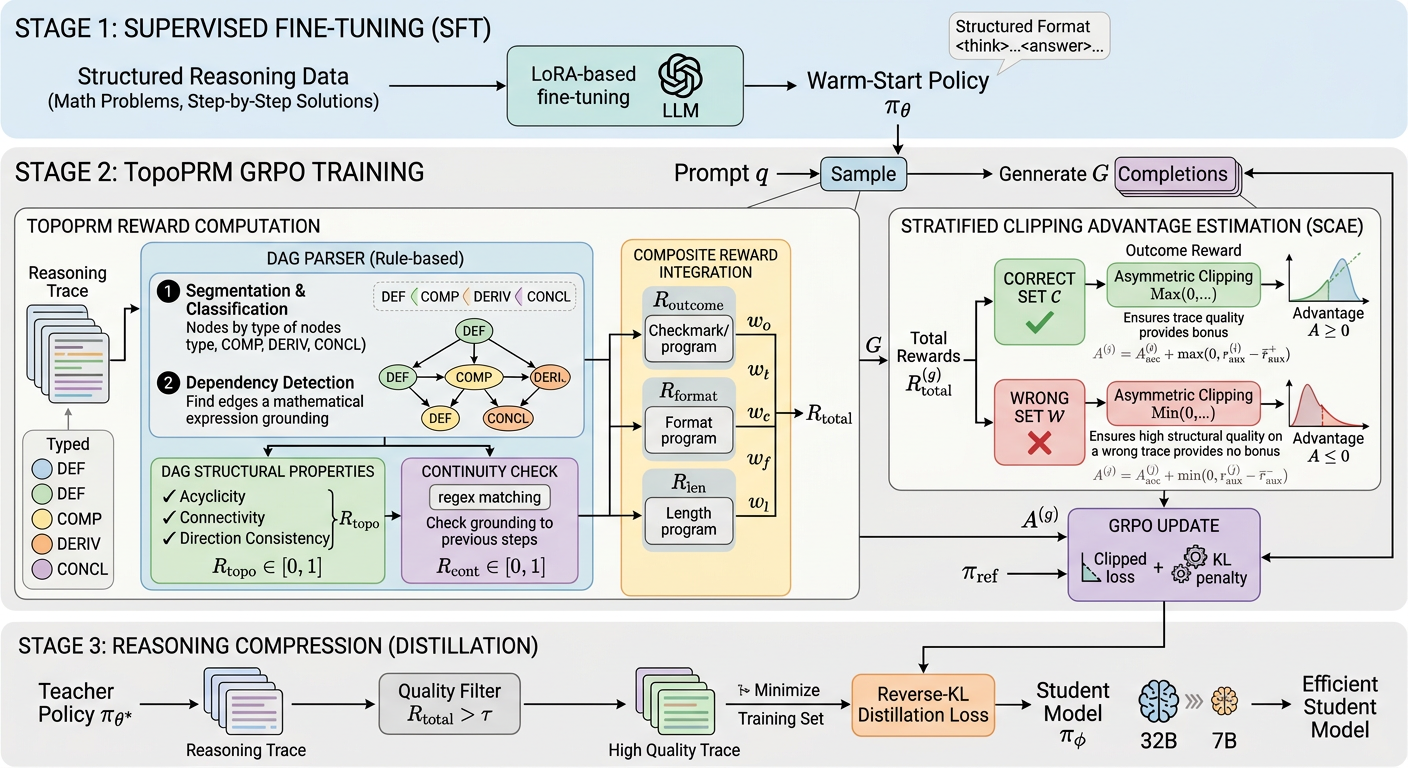
\includegraphics[width=0.98\linewidth]{figures/Ai_Framework.png}
    \caption{Overview of \method. The same dependency DAG extractor feeds three pillars: topology-aware data processing produces structural diagnostics from each trace; a hierarchical reward aggregation combines outcome, topology, and continuity signals during GRPO training; and a topology-guided self-distillation stage reuses the same diagnostics to compress long-CoT teachers into compact students.}
    \label{fig:overview}
\end{figure*}

\method is a topology-aware post-training framework with one shared dependency-DAG extractor (Figure~\ref{fig:overview}).
The framework, which we call \framework, consists of three sequential post-training stages that share the same DAG-based supervision interface:
\textbf{Stage~I} supervised fine-tuning (SFT) for cold-start format compliance;
\textbf{Stage~II} group relative policy optimization (GRPO) with our hierarchical multi-source reward, where outcome correctness forms the top layer and the topology-sensitive diagnostics $q_{\mathrm{topo}},q_{\mathrm{cont}}$ (derived from the DAG Scorer, constituting our \prm) are combined with format and length signals, and advantages are estimated using Stratified Clipping Advantage Estimation (\estimation);
\textbf{Stage~III} \emph{Topology-Guided On-Policy Distillation} (TG-OPD), where the Stage-II teacher provides token-level RKL supervision while the student rolls out its own trajectories under topology-conditioned revision prompts.
Using one extractor across all stages gives a single, auditable structural supervision interface instead of separate heuristics for training and compression.

\subsection{Problem Setup}

Given an input $x=(q,s)$, where $q$ is a problem and $s$ is optional context, a policy $\pi_\theta$ generates a reasoning trace $y \sim \pi_\theta(\cdot\mid x)$.
Outcome-only training supervises $y$ with a sparse final-answer signal $r_{\mathrm{out}}(x,y)\in\{0,1\}$.
This signal is sufficient for end answers, but it cannot distinguish unsupported conclusions, spurious linearized dependencies, and structurally redundant branches.
Our objective is to recover latent dependency structure from $y$ and use it as unified supervision across SFT, RL, and distillation without human step labels or learned verifier models.

\subsection{Topology-Aware Data Processing}
\label{sec:reward_module}

\subsubsection{Trace-to-DAG extraction and diagnostics}
For a trace $y=(s_1,\ldots,s_T)$, we apply a deterministic extractor
$\mathcal{G}=\mathcal{E}(y)=(\mathcal{V},\mathcal{A})$, where each node is a reasoning step and each directed edge denotes rule-based dependency evidence (expression reuse, claim reference, or structural connector).
The extractor performs step segmentation, claim normalization, and edge construction with explicit fallbacks for unsupported derivation steps.
To reduce parser artifacts, claim extraction uses sentence-level units and filters incomplete heading-like fragments before matching.

From $\mathcal{G}$ we compute two reward-facing structural signals:
global topology quality $q_{\mathrm{topo}}\in[0,1]$ and local continuity quality $q_{\mathrm{cont}}\in[0,1]$.
$q_{\mathrm{topo}}$ summarizes acyclicity, orphan-conclusion support, direction consistency, and optional reference-edge alignment, capturing \emph{latent conditional dependencies} surfaced by expression and claim reuse.
$q_{\mathrm{cont}}$ measures step-level support traceability along the weak sequential edges, capturing \emph{ordered continuity} that outcome-only supervision leaves unobserved.
Both are produced by the same deterministic pipeline, so they act as a \emph{topology-sensitive \prm}: step-level signals that require neither human annotations nor a learned verifier, and remain fully auditable on any rolled-out trace. We treat this \prm as a structural sub-component of \method, on top of which the hierarchical reward in \S\ref{sec:post_training} is built.
We report full definitions and term-level equations in Appendix~\ref{app:math_details}.

%\subsubsection{Scope of Verifiability}
% See Appendix for extended discussion on reward aggregation strategies.
% Our use of ``verifiable'' is operational: once a trace is produced, all reward values are computed by deterministic procedures and are therefore reproducible and auditable.
% This is distinct from semantic proof verification; we do not claim step-correctness guarantees or logical completeness.

\subsection{Three-Stage Post-Training Framework}
\label{sec:post_training}
The three stages of \framework share a single DAG-based supervision interface.
Stage~I (SFT) aligns format and basic reasoning behaviour, Stage~II (GRPO with hierarchical reward) injects topology-sensitive process supervision without overriding answer correctness, and Stage~III (TG-OPD) reuses the same diagnostics for compact-student distillation.
Unlike linear reward mixing, we preserve outcome primacy in Stage~II and inject process supervision as a multiplicative structural gain.

\subsubsection{Stage~I: SFT Cold-Start}

We fine-tune the base model on a mixture of mathematical critique examples and public-domain math reasoning problems to establish basic format compliance and reasoning behaviour.
Critique data accelerates format adaptation but is not the target distribution for public math benchmarks, so the SFT checkpoint $\pi_\theta$ is treated as an initialisation for reinforcement learning rather than as a deployable reasoner.

\subsubsection{Stage~II: GRPO with Hierarchical Reward Aggregation}

Each training step samples completions from $\pi_\theta$, extracts dependency DAGs, and computes five reward signals: outcome correctness $r_{\mathrm{out}}$, format compliance $r_{\mathrm{fmt}}$, length penalty $r_{\mathrm{len}}$, and the structural diagnostics $q_{\mathrm{topo}}$ and $q_{\mathrm{cont}}$ defined in \S\ref{sec:reward_module}.

\paragraph{Hierarchical aggregation.}
Weighted-sum rewards can mis-rank traces when high process scores compensate for wrong answers~\citep{Denison2024SycophancyTS}, and they are prone to reward-variance collapse in group-relative RL~\citep{yu2025dapo,kazemnejad2025vineppo}.
We therefore separate correctness base reward from structural gain:
\begin{equation}
\label{eq:r_total}
r_{\mathrm{total}} =
\bigl(w_o r_{\mathrm{out}} + w_f r_{\mathrm{fmt}} + w_l r_{\mathrm{len}}\bigr)
\cdot
\bigl(1 + \alpha q_{\mathrm{topo}} + (1-\alpha) q_{\mathrm{cont}}\bigr),
\end{equation}
where $r_{\mathrm{out}}$ is outcome correctness, $r_{\mathrm{fmt}}$ is format compliance, and $r_{\mathrm{len}}$ is length regularization.
$q_{\mathrm{topo}}$ and $q_{\mathrm{cont}}$ are normalized structural diagnostics from the extracted DAG.
$\alpha\in[0,1]$ controls topology/continuity balance.
This form preserves correctness primacy while enabling structural differentiation among outcome-equivalent traces.

\paragraph{Anti-collapse mechanisms.}
To reduce reward collapse in GRPO, we use batch-relative normalisation and correctness-first shaping, and monitor low-variance groups while retaining a positive base floor so that process gains do not vanish when outcome rewards are sparse. As an additional safeguard against multiplicative reward hacking, we follow \citet{liu2026graph} and estimate advantages with stratified clipping (\estimation), which partitions each GRPO group by correctness and bounds the auxiliary contribution of $q_{\mathrm{topo}}$ and $q_{\mathrm{cont}}$ within each stratum so that structural scores cannot flip the sign of an outcome-wrong trace:
\begin{equation}
\label{eq:scae}
\widehat{A}_i \;=\;
\mathrm{clip}\!\Big(\tfrac{R_i-\mu_{\mathcal{B}^{\pm}}}{\sigma_{\mathcal{B}^{\pm}}+\epsilon},\,
\,\underline{c}^{\pm},\,\overline{c}^{\pm}\Big),
\qquad i\in\mathcal{B}^{\pm}.
\end{equation}
Implementation and ablation of \estimation, together with diagnostics for the anti-collapse monitors, are reported in Appendix~\ref{app:scae}.

\subsection{Stage~III: Topology-Guided On-Policy Distillation}
\label{sec:compression}
\label{sec:tgsd}

Stage~III reuses the same DAG diagnostics to compress the long-CoT teacher $\pi_T$ (obtained from Stage~II) into a compact reasoning student $\pi_S$.
We call this procedure \emph{Topology-Guided On-Policy Distillation} (TG-OPD): the student rolls out its own trajectories, the teacher provides token-level supervision, and the DAG extractor $\mathcal{E}$ issues topology-conditioned revision prompts that localise where supervision should focus.
Since the teacher is the Stage-II \method checkpoint rather than an external reference, TG-OPD instantiates the ``self-distillation'' aspect of \framework at the framework level.

Off-policy reverse-KL distillation~\citep{hinton2015distilling,minillm2023} often inherits teacher verbosity and format failures under long-generation budgets; recent on-policy distillation work attributes the same failure to train-test mismatch~\citep{agarwal2024gkd,opsdc2026,song2026opdsurvey}.
We therefore perform on-policy distillation conditioned on topology diagnostics.
Given an initial response $y_{\mathrm{init}}$ from the student, we compute $(r_{\mathrm{out}}, q_{\mathrm{topo}}, q_{\mathrm{cont}})$ via $\mathcal{E}$ and generate a revision instruction
$P_r=\psi(r_{\mathrm{out}},q_{\mathrm{topo}},k)$, where $k$ is sampled from orphan-conclusion diagnostics.
The full prompt dispatch and filtering criteria are given in Appendix~\ref{appx:tgsd_details}.

\paragraph{Structural view: from layered DAG to a compact chain.}
The extracted DAG admits a deterministic linearization that drives what we want the student to imitate.
Same-type consecutive steps are merged into macro-nodes (step-type contraction), topologically parallel branches are folded into layers, and transitively redundant edges are removed, leaving a compact chain that follows the \emph{critical dependency path} from premises to conclusion, a graph-theoretic analogue of critical-path analysis in project scheduling.
This view makes the supervision target explicit: rather than matching teacher token frequencies, the student should recover the shortest structurally supported trajectory that closes the answer, so compression reduces redundant branches and token budget instead of collapsing dependency structure.

The student objective is topology-conditioned token-level reverse KL:
\begin{equation}
\label{eq:tgsd}
\mathcal{L}_{\text{TG-OPD}} =
\mathbb{E}_{x\sim\mathcal{D}_2,\,y\sim\pi_\theta(\cdot\mid x)}
\sum_{t=1}^{|y|}
D_{\mathrm{KL}}\!\left(
\pi_\theta(\cdot\mid x,y_{<t})\,\bigg\|\,
\pi_{\mathrm{ref}}(\cdot\mid x,y,P_r,y_{<t})
\right).
\end{equation}
Conditioning on $P_r$ focuses supervision on structurally suspect regions (for example orphan conclusions and continuity breaks), so compression preserves dependency structure instead of only matching teacher token frequencies.
Here the teacher $\pi_{\mathrm{ref}}$ is the Stage-II \method checkpoint and contributes long-CoT rollouts and topology-aware revision targets, while the student $\pi_\theta$ generates on-policy trajectories that are pushed toward shorter, structurally supported chains; the dependency DAG on both sides is always produced by the same deterministic extractor $\mathcal{E}$ rather than by either model.

\begin{algorithm}[!htb]
\caption{\framework Training Pipeline (SFT $\to$ GRPO $\to$ TG-OPD)}
\label{alg:topoprm}
\begin{algorithmic}[1]
\Require Base $\pi_0$, SFT data $\mathcal{D}_{\mathrm{sft}}$, RL prompts $\mathcal{D}_{\mathrm{rl}}$
\Ensure Teacher $\pi_T$, verifier $\pi_{\mathrm{ref}}$, compact student $\pi_S$
\State $\pi_\theta \leftarrow \mathrm{SFT}(\pi_0,\mathcal{D}_{\mathrm{sft}})$ \Comment{Stage~I: cold-start}
\For{each GRPO batch on $\mathcal{D}_{\mathrm{rl}}$} \Comment{Stage~II}
  \State Sample completions; extract DAGs via $\mathcal{E}$
  \State Compute $r_{\mathrm{out}},r_{\mathrm{fmt}},r_{\mathrm{len}},q_{\mathrm{topo}},q_{\mathrm{cont}}$
  \State Aggregate by Eq.~\ref{eq:r_total}; estimate advantages with \estimation
  \State GRPO update on $\pi_\theta$
\EndFor
\State $\pi_T \leftarrow \pi_\theta$ \Comment{Stage-II teacher checkpoint}
\If{TG-OPD enabled} \Comment{Stage~III}
  \State Initialize student $\pi_S$ from a smaller pretrained model
  \For{each batch of prompts $x$ in $\mathcal{D}_{\mathrm{rl}}$}
    \State $y_{\mathrm{init}} \sim \pi_S(\cdot\mid x)$ \Comment{on-policy rollout}
    \State $\mathcal{G}_{\mathrm{init}} \leftarrow \mathcal{E}(y_{\mathrm{init}})$; compute $(r_{\mathrm{out}}, q_{\mathrm{topo}}, q_{\mathrm{cont}})$
    \State $P_r \leftarrow \psi(r_{\mathrm{out}}, q_{\mathrm{topo}}, k)$ \Comment{revision prompt from orphan-conclusion diagnostics}
    \State $y_{\mathrm{rev}} \sim \pi_T(\cdot\mid x, y_{\mathrm{init}}, P_r)$ \Comment{teacher revision under topology prompt}
    \State Discard samples that violate format or fail topology filters
    \State Update $\pi_S$ by minimising the token-level reverse KL in Eq.~\ref{eq:tgsd}
    \Statex \hspace{1em}\textit{(optional structural view: layer-compress $\mathcal{G}$ to its critical dependency chain as an auxiliary supervision target)}
  \EndFor
\EndIf
\State \Return $(\pi_T, \pi_S)$
\end{algorithmic}
\end{algorithm}

